\chapter{Background Theory}

% \newenvironment{conditions}
%   {\par\vspace{\abovedisplayskip}\noindent\begin{tabular}{>{$}l<{$} @{${}={}$} l}}
%   {\end{tabular}\par\vspace{\belowdisplayskip}}
  
\newenvironment{conditions}[1][where:]
  {#1 \begin{tabular}[t]{>{$}l<{$} @{${}={}$} l}}
  {\end{tabular}\\[\belowdisplayskip]}

\label{ch:background}

\section{Concepts of Causality}
\label{concepts}

Current supervised Machine Learning techniques are designed to exploit possible relationships/correlations between features and labels in order to produce reliable estimates. Use of this kind of technologies in ambit such as Medicine, Finance and Law are now raising increasing concerns due to the lack of ability in such systems to correctly identify causal relationships and provide explanations about their decisions. One possible solution in order to overcome these type of problems if by taking into account causal relationships.

Causality arises naturally in our daily life every-time we ask ourselves any type of interventional or retrospective question (eg. What if I take this action? What if I would have acted differently?).

As shown in Figure \ref{pyr}, Causal Reasoning can be divided in three different hierarchical levels (Association, Intervention, Counterfactuals). At each level, different types of questions can be answered and in order to answer questions at the top levels (eg. Counterfactuals) are necessary as basis knowledge from the lower levels \cite{tools}. In fact, in order to be able to able to answer retrospective questions, we would expect to first be able to respond to intervention and association type of questions.

\begin{figure}[ht!]%
    \centering
    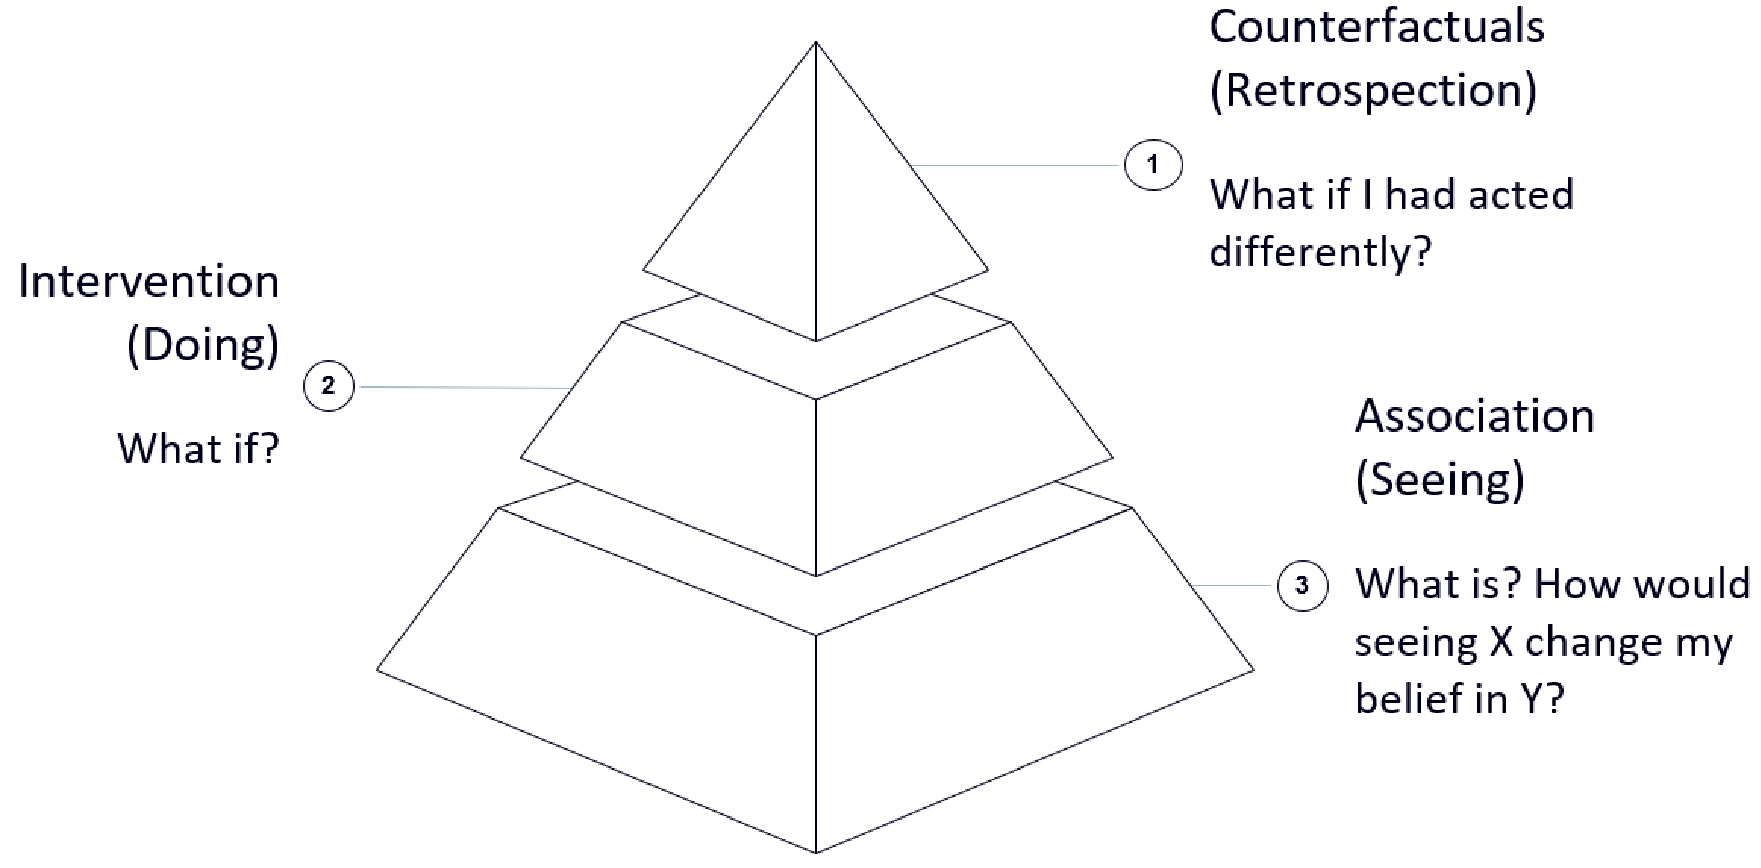
\includegraphics[width=0.8\linewidth]{latex/images/pyramid.pdf}
    % 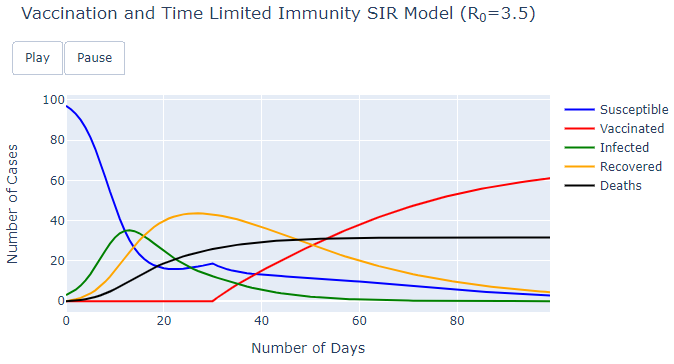
\includegraphics[width=13cm]{latex/images/vacc.PNG}%
    \vspace{-0.2cm}
    \caption{Causality Hierarchy}
    \label{pyr}
\end{figure}
\vspace{-0.5cm}

Currently, Machine Learning models are only able to answer the probabilistic type of questions related to the Association level.
Thanks to the rising interest in this topic, a mathematical framework able to represent causal relationships has been constructed (Structural Causal Models (SCM) \cite{tools}). Using this type of framework, causal expressions can then be formulated and used in conjunction with data in order to make predictions.

This type of framework, can then be divided into two main parts: causal diagrams and a symbolic language. The causal diagrams can be used in order to summarise our knowledge about the topic, while the symbolic language can be used to express what we are aiming to find out.

As an example, let us consider the diagram shown in Figure \ref{dig_ex}. Using this type of representation, the arrow directions indicate how the different variables effects each other.

In this example, a survey is carried out between individuals of age 3-20 in order to find out if there is any correlation between height and Individuals Intelligence Quotient (I.Q.) Scores. Although the study might result in a positive correlation between the two different variables, a more in depth analysis might instead show how height does not directly cause higher I.Q. Scores but these two variables are instead dependent on a third hidden variable (Confounder). In fact, as children grow up, over time both their I.Q. Scores and height tends to increase thanks to their improved education and greater age.  

\begin{figure}[ht!]%
    \centering
    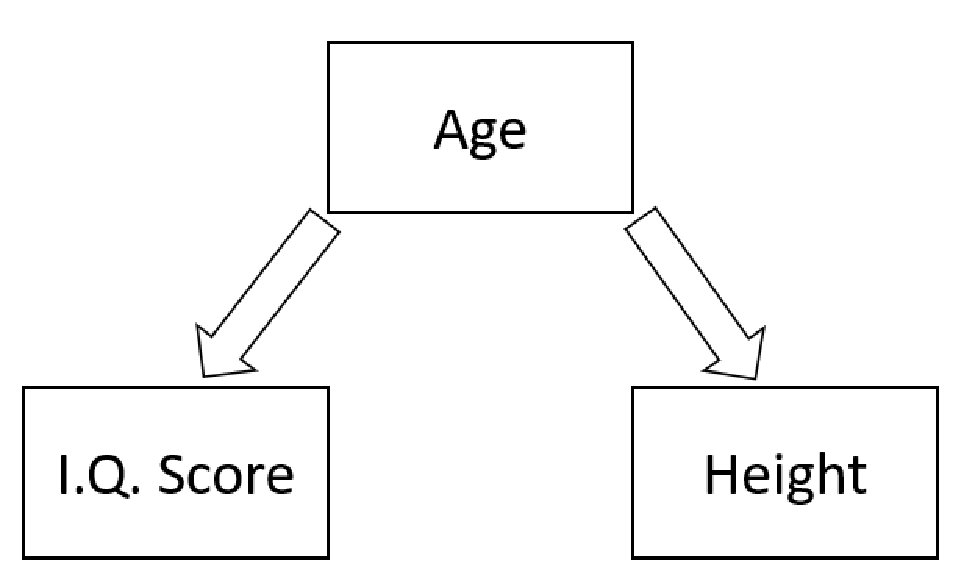
\includegraphics[width=0.4\linewidth]{latex/images/caus_d.pdf}
    \vspace{-0.2cm}
    \caption{Causality Diagram}
    \label{dig_ex}
\end{figure}
\vspace{-0.5cm}

In case we want to query additional information from what we currently have available \footnote{So that to move from the association to the intervention level in the causality hierarchy.}, we can then make use of the symbolic language in order to advance questions such as: What is the probability (P) that a student will get an higher I.Q. score (S) if he studies an additional amount of time (T)? This question could then be formulated in a symbolic form such as $P(S|do(T))$  \footnote{Although, Do-Calculus notation might look similar to the one of conditional probability, the two have two different meanings.}. When formulating these type of questions, we are then implying that we are not anymore passively observing possible results but instead actively intervening in order to find out about possible consequences. This type of approach is known as an Interventional Study and is in contrast with traditional Observational Studies.

Finally, in order to create a full Causal Inference Engine, an architecture like in Figure \ref{engine}, might be necessary \cite{why}. Following this type of approach, three inputs are needed and three outputs are produced. As our three inputs, are given any assumption made about the model (\textbf{Assumptions}), any questions we are trying to answer (\textbf{Queries}) and any data which can be used in order to fuel our engine (\textbf{Data}). The model, will then output as Boolean value if is able or not to answer the given queries, and if so, it would provide as second output a mathematical formula which can be used in order to answer the queries. Finally, a numerical prediction specific to the given input data is provided (this might contain some form of uncertainty in the estimation given the amount of data provided and the assumption made).  

\begin{figure}[ht!]%
    \centering
    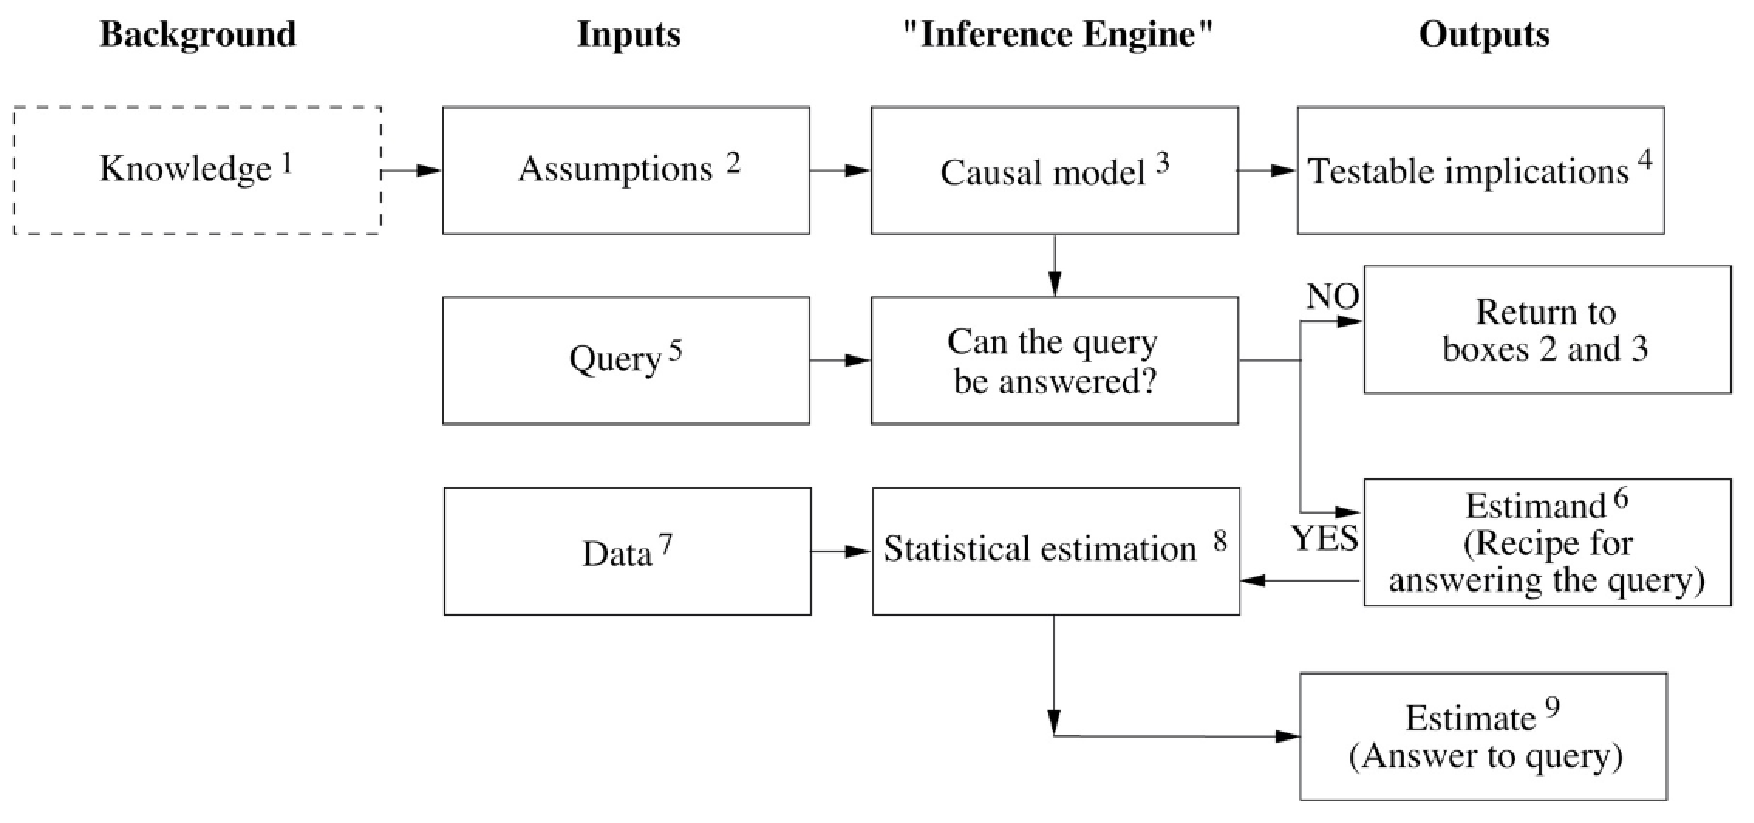
\includegraphics[width=0.8\linewidth]{latex/images/engine.pdf}
    \vspace{-0.2cm}
    \caption{Causal Inference Engine (Image reproduced from: \cite{why})}
    \label{engine}
\end{figure}
\vspace{-0.5cm}

Using this type of paradigm, can ultimately make our model much more flexible than contemporary deep learning models (in fact, our model is now much less dependent on the data and more focused about intrinsic relationships and connections).

\section{Linear and Non-Linear Causality}
\vspace{-0.1cm}
Causality, can be divided into two main types: linear and non-linear (Figure \ref{wow}) \cite{system}: 
\vspace{-1.3cm}
\begin{itemize}
    \setlength\itemsep{-0.5em}
    \item In linear causality, connections between the variables can be in a single direction and every effect can be originated by a limited number of causes. Causes always linearly precedes effects (time precedence).
    \item In non linear causality, connections between variables can be bi-directional and effects can possibly be originated by an unlimited number of causes.
\end{itemize}
\vspace{-0.4cm}
Linear causation systems are characterised by proportional relationships between cause and effects variables (e.g. Deterministic Systems). Instead, in non-linear causation systems disproportionate effects can take place (e.g. Non-deterministic Systems). For example, small changes in input conditions would then result in different consequences (e.g. "Butterfly Effect").
\vspace{-0.1cm}
\begin{figure}[ht!]%
    \centering
    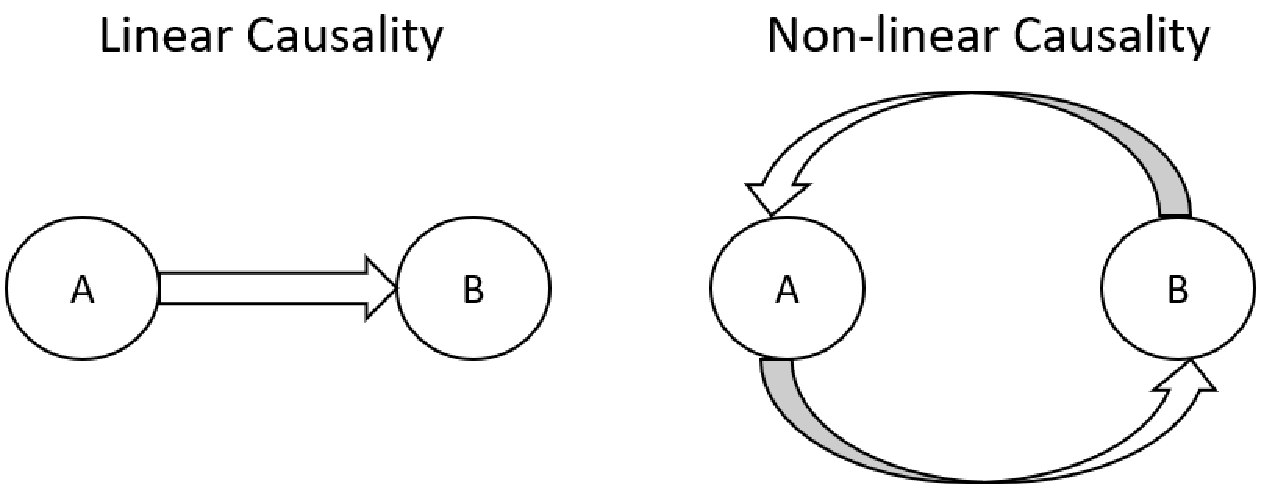
\includegraphics[width=0.7\linewidth]{latex/images/linear.pdf}
    % 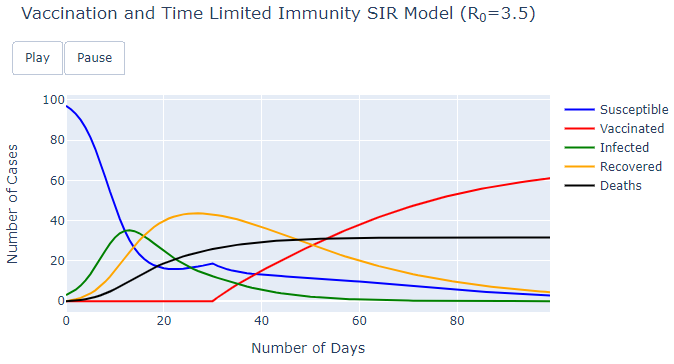
\includegraphics[width=13cm]{latex/images/vacc.PNG}%
    \vspace{-0.2cm}
    \caption{Linear vs Non-Linear Causality}
    \label{wow}
\end{figure}
\vspace{-0.5cm}

From an external point of view, each causal systems can then be characterised as a composition of events, which although might be regulated by a series of hidden trends and rules. Being able to correctly identify how these different constituent forces are interconnected each other (grasping any reciprocal causal mechanism), would then allow us to make any system much more predictable. 

The causal analysis of any dynamical system, could then be summarised by the following workflow (Figure \ref{wow2}). 

\begin{figure}[ht!]%
    \centering
    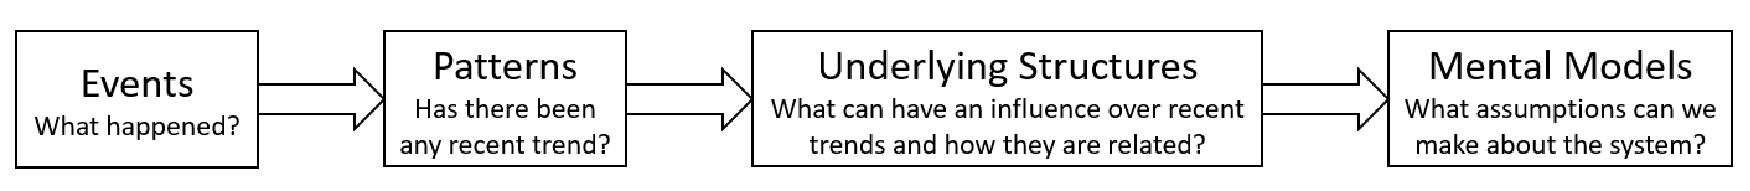
\includegraphics[width=1\linewidth]{latex/images/discover.pdf}
    % 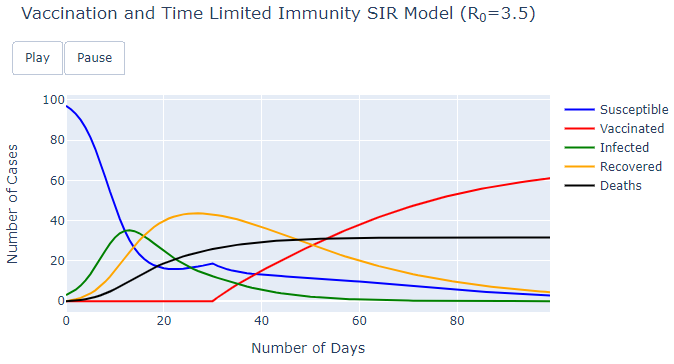
\includegraphics[width=13cm]{latex/images/vacc.PNG}%
    \vspace{-0.6cm}
    \caption{Dynamical Systems Analysis (Adapted from \cite{system})}
    \label{wow2}
\end{figure}
\vspace{-0.5cm}

\section{Bayesian Belief Networks}
\label{bbn_ref}
Bayesian Belief Networks (BBN), are a type of probabilistic model which makes use of simplifying assumptions so that to reliably define connections between different elements and calculate their probabilities relationships efficiently. By analysing interactions between the different elements, we can finally make use of these type of models in order to discover causal relationships. 

In a Bayesian Network, nodes represent variables while edges report the probabilistic connections between the different elements. A simple example of a three variables Bayesian Belief Network, is available in Figure \ref{net}. 

\vspace{-0.5cm}
\begin{figure}[ht!]%
    \centering
    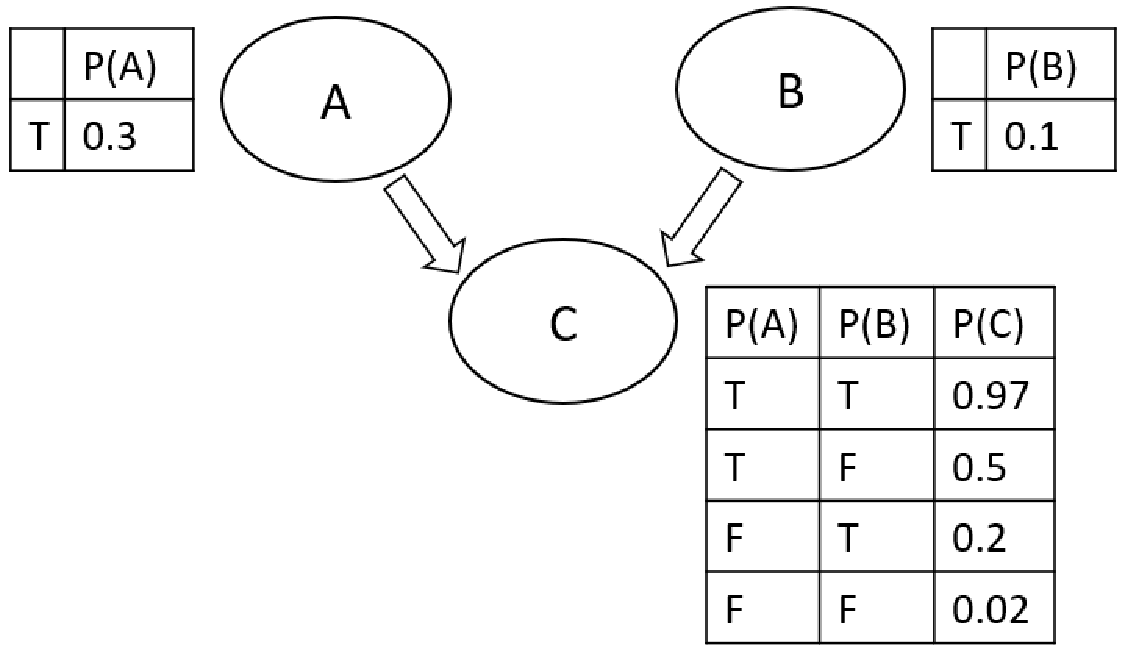
\includegraphics[width=0.7\linewidth]{latex/images/bayes.pdf}
    % 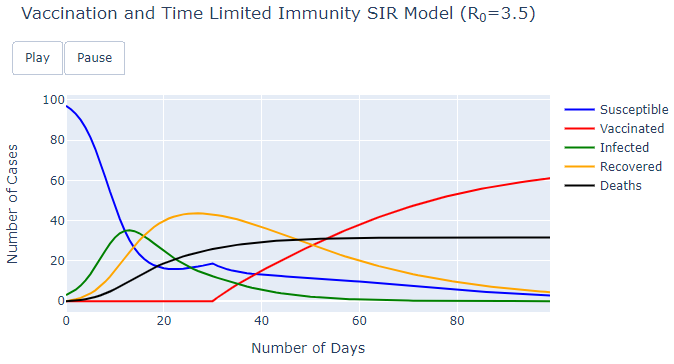
\includegraphics[width=13cm]{latex/images/vacc.PNG}%
    \vspace{-0.2cm}
    \caption{Bayesian Belief Network}
    \label{net}
\end{figure}
\vspace{-0.7cm}

Bayesian Belief Networks, led later on to the development of Causal Networks. In fact, they can also be considered as a Causal Network in some specific cases. For this reason, Bayesian Belief Networks are nowadays considered to be one of the main techniques which can be used in Machine Learning in order to move from the Association to the Intervention level in the Causality Hierarchy (Figure \ref{pyr}).

Bayesian Belief Networks, are able to express both conditional dependent and independent variables connections. These type of networks, follow additionally the Markov condition \cite{markov} (provided the parents of every node in a network, each node is conditionally independent of their nondescendent nodes).  Finally, using Bayes probabilistic approach (Equation \ref{beq}), we can be able to update the connection probabilities iteratively based on new gathered evidence.

\useshortskip
\begin{equation}
P(A|B) = \frac{P(B|A)\times P(A)}{P(B)}
\label{beq}
\end{equation}
\vspace{-0.2cm}
\begin{conditions}
 $A,B$   &  Events \\
 $P(B|A)$ &  Likelihood \\
 $P(A)$   &  Prior \\   
 $P(B)$ & Normalizing Constant \\
 $P(A|B)$ & Posterior
\end{conditions}
\useshortskip

Complex BBNs can be constructed by starting from three basic types of junctions: Chains (e.g. $A \Rightarrow B \Rightarrow C$), Forks (e.g. $A \Leftarrow B \Rightarrow C$) and Colliders (e.g. $A \Rightarrow B \Leftarrow C$). Making use of the three types of junctions and of a technique called d-separation, it can then be possible to reach the Counterfactuals level in the Causality Hierarchy \cite{why}. D-separation, allow us in fact to understand, in Causal Diagrams, if a set of variables is independent of another set when given a third one. 

What distinguishes Bayesian statistic from the classical frequentistic approach, is that we allow to incorporate some level of subjectivity in our model\footnote{Frequentistic probability aims instead for complete objectiveness.} (by combining prior knowledge with evidences). Additionally, in Bayesian statistics, the weight of our prior belief gradually vanishes as more data is provided (therefore converging to the frequentistic approach if given an unlimited amount of data). This case, doesn't instead hold true when talking about causality analysis.

Great research focus by companies such as DeepMind is currently put into using Bayesian Belief Networks as starting point in order to create Causal Bayesian Networks (CBN) \cite{deep}. Causal Bayesian Networks, are nowadays used in order to visually identify and quantitatively measure unfairness patterns in datasets (elements in the data which can lead to Machine Learning models biased towards specific subcategories). Additionally, researches also demonstrated the possibility to use Causal Bayesian Networks in order to identify if not just the data but also the Machine Learning models itself are biased or not towards specific classes \cite{deep2}.

\section{Intervention}
What allow us to talk about cause and effect, are experiments. Experiments, are a set of procedures carried out under controlled conditions, so that to test an hypothesis and try to undercover causes. Controlling the conditions of an experiment, can allow us in fact to eliminate any alternative explanations which we might have about the how a phenomena works. When creating an experiment, we need to make sure that different treatments are applied and that they are randomly assigned \cite{cassie}. In an experiment, a treatment is defined to be as a change imposed from us to the environment of the experiment. Treatments, should additionally be randomly assigned in order to make up for any variability in the environment space (e.g. different individuals/objects might have different characteristics). Finally, if working with just a sample from a population, it is necessary to make sure that the available sample size is large enough to be representative of the whole population. If all these characteristics are provided, then we can be able to accurately discover causal relationships even under uncertainty. Therefore, experiments play a key role in order for us to move between the different levels in the Causality Hierarchy (Figure \ref{pyr}). If any of the conditions, doesn't instead hold true, we might end up accidentally adding some form of bias in our experiment. Without experiments, data driven decisions can just be backed by correlations and domain knowledge, but no pure evidences.

One of the main differences between Causal Diagrams and Bayesian Belief Networks, is that the former are able to deal with interventions, while the latter works only with observations. Interventions allows us to use Causal Inference, while observations allows us to make predictions. What makes possible for Causal Diagrams to work with interventions is the Do Operator. From the Do Operator, has then been possible to create the Do Calculus which has been demonstrated to be complete as a technique (if Do Calculus is not able to identify an effect, then this cannot be identified anywhere else). On the other hand, what makes difficult to use Causal Diagrams is making sure they are designed correctly. In fact, different Causal Diagrams can potentially be proposed in order to describe a process and depending from different point of views, it can be difficult to understand which one is able to better capture the underlying dynamics of a process.

For example, let's imagine we have carried out a study in order to find out if a diet can bring a positive effect (above the average) on the overall well-being of a sample in a population. Therefore, we divide the participants of this experiment into two groups: one which will strictly follow the diet and the other one which will instead follow common used diet-lifestyles. From this study might result that following the diet causes a positive effect to the individuals well-being (Figure \ref{cex1}).

\begin{figure}[ht!]%
    \centering
    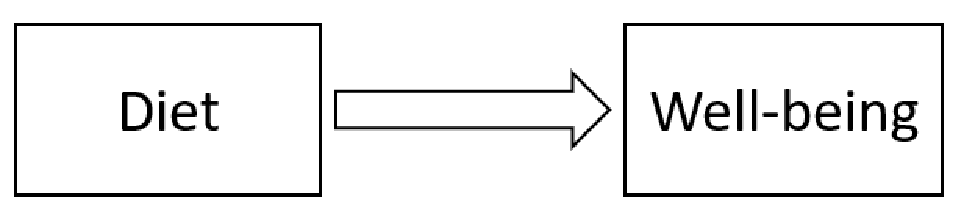
\includegraphics[width=0.4\linewidth]{latex/images/simple_ex.pdf}
    % 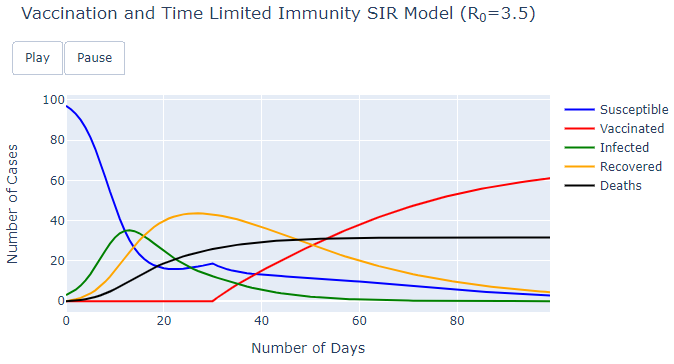
\includegraphics[width=13cm]{latex/images/vacc.PNG}%
    \vspace{-0.2cm}
    \caption{Simple Causal Diagram}
    \label{cex1}
\end{figure}
\vspace{-0.5cm}

Although, at this point we might start having some doubts about if there could be any potential pitfall in our analysis. One possible approach in order to test for the presence of confounding variables is to take measurements about the suspected hidden variable (in this way, we can be able to fill any missing piece in our diagram). Carrying out a controlled experiment, we will be able to deconfound any true and "spurious" effect this hidden variable might cause. In the case of our example, we could for instance notice that the group which followed the diet had an overall younger age than the other group. Therefore, age could be considered as a possible factor which has skewed our early results and that we should therefore take into account (Figure \ref{cex2}).  

\begin{figure}[ht!]%
    \centering
    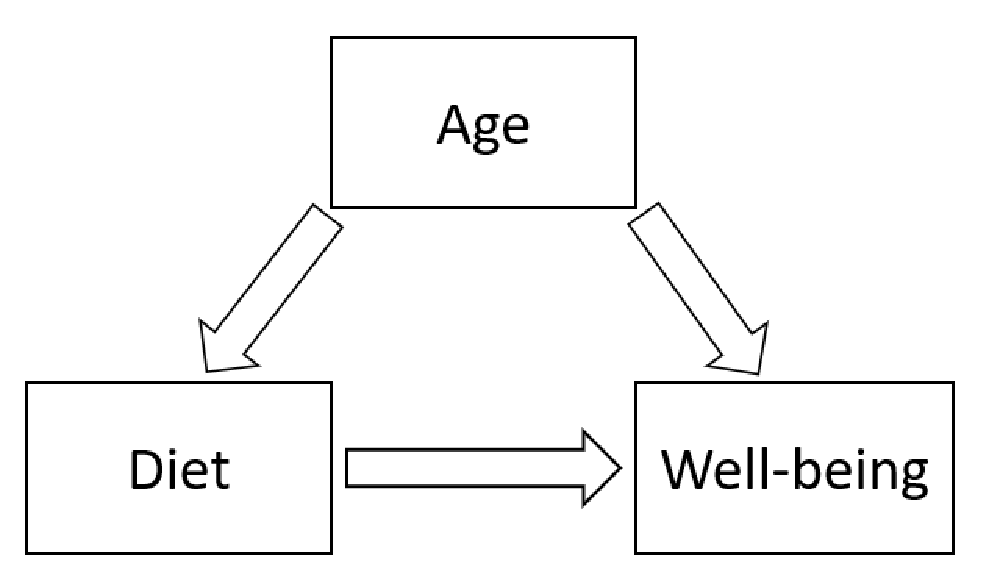
\includegraphics[width=0.4\linewidth]{latex/images/simple_ex2.pdf}
    % 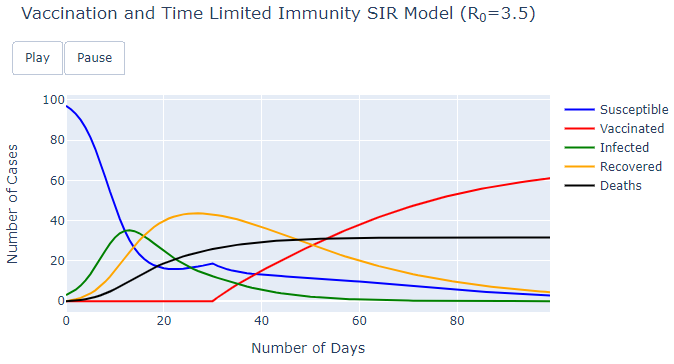
\includegraphics[width=13cm]{latex/images/vacc.PNG}%
    \vspace{-0.2cm}
    \caption{Improved Causal Diagram}
    \label{cex2}
\end{figure}
\vspace{-0.5cm}

Our confounding variable (Age) could then be deconfounded by comparing the two different groups of the experiment for different age groups, averaging the results and weight the different age groups sections by their percentage presence in the population composing the experiment. This procedure is commonly referred as \textbf{adjusting/controlling for a variable} \cite{why}. Examining the results of our analysis we could then maybe think there might be some other variables missing and repeat this process again to improve our representation of the system. A confounding, can therefore be defined to be as anything making $P(A|B)$ different from $P(A|do(B))$.   

In a causal diagram, information can flow through links from one vertex to another in two different directions (causal and noncausal). In this setting, information flowing in the noncausal direction, can then lead to the creation of confoundings. In order to avoid this problem, information flowing in the noncausal direction can be blocked by using either of the following three approaches:

\begin{itemize}
    \item Accurate controlled experiment randomization.
    \item Statistical variable adjustments.
    \item Applying the Do Operator on a variable, can stop the flow of information in the noncausal direction (this procedure can also be applied when working with observational data).
\end{itemize}

Finally, information flow in causal diagram is regulated by the same type of junctions introduced in Section \ref{bbn_ref}. Controlling for different variables in these types of junctions (to prevent presence of confoundings), would then lead to the following results:

\begin{itemize}
    \item \textbf{$A \Rightarrow B \Rightarrow C$}: controlling $B$ would stop information to flow between $A$ and $C$.
    \item \textbf{$A \Leftarrow B \Rightarrow C$}: like in the previous case, controlling $B$ would stop information to flow between $A$ and $C$.
    \item \textbf{$A \Rightarrow B \Leftarrow C$}: controlling $B$ would in this case enable information to flow between $A$ and $C$ (without intervention, no information would have been able to flow).
\end{itemize}

Making use of this set of information, can then be possible to create and work with a multitude of different causal diagrams.

\vspace{-0.2cm}
\subsection{A/B Testing}
\label{testing}
\vspace{-0.2cm}
A/B Testing is one of the most common form of experimentation in Computer Science. Companies nowadays make common use of A/B Testing for instance when shipping a new feature in production. For example, a company might come up with a new design for a section on an App. To a randomised half of the users is going to be proposed the new version (Treatment Group), while to the other half is going to be proposed the original version (Control Group). Collecting users behaviours and feedback could then be possible to observe the causal effects of our interventions. This type of approach can be considered to be analogous to how vaccines/drugs are evaluated in clinical trials.

\section{Counterfactuals}
Carrying out experiments can be difficult and expensive in different real-life situations, in that case, we can perform just observational studies (we don't exercise any control on our independent variable). When working with observational data, changes between the control and treatment groups become \textbf{counterfactual} therefore making difficult to undercover causal effects. Due to these limiting circumstances, it is then necessary to make some assumptions in order to create an approximation model able to make predictions. Counterfactual analysis focuses then on how different types of interventions could have retrospectively led to different outcomes (imagining alternative "worlds"). 

Some examples of Counterfactuals types of questions are: Would the patient have survived whiteout taking any medication? How likely it is that a political party would have won the elections if it had proposed a more liberal policy than the advertised one? 

Because of the nature of these types of questions, it can be difficult to provide answers with full certainty. Therefore, some form of probabilistic mechanism needs to be incorporated (e.g. We are 90\% confident that choosing a more liberal policy would have increased the chances of winning the elections by 7\%).

This type of probabilistic approach can be introduced by using \textbf{potential outcomes}. Potential outcomes are determined on an individual level (not with respect of the entire population) and they depend on the assumption that if a value if assigned to a first variable, then a value should be assigned to its dependent variables \cite{why}.

One of nowadays main application of Counterfactuals, is \textbf{mediation analysis}. Mediation analysis is based on the concept of mediating variables (variables used to influence an outcome based on the effect of an applied treatment). An example of a mediating variable can be $Vitamin\:A$ in $Eating\:Carrots \Rightarrow Vitamin\:A \Rightarrow Improved\:Eye\:Sight$. The aim of mediation analysis in this setting would then be to understand if the mediating variable is able to capture all the effects caused by the treatment variable ($Eating\:Carrots$) or not. Effects can then either reach our outcome variable directly or indirectly (through the mediating variable). Direct effects could then be represented in our example as moving through the following diagram without the need of mediating variables: $Eating\:Carrots \Rightarrow Improved\:Eye\:Sight$. Using mediation analysis we could then be able for example to find out if eating carrots is possible to improve our eye sight just by the increase of Vitamin A resources or through any other effect.

What makes mediation analysis an interesting field of research, is the fact that the total effect exercised by a variable is not simply equal to the sum of its exercised direct and indirect effects in the case of third party variables interactions.

Examples of other techniques ideated during the course of the last decade in order to try to solve Counterfactual problems are \cite{eva}:

\begin{itemize}
    \item \textbf{Do Calculus}
    \item \textbf{Ordinary Least Squares with Confounding Variables}
    \item \textbf{Propensity Score Matching}
    \item \textbf{Instrumental Variables}
    \item \textbf{Difference in Differences}
\end{itemize}

\section{Case Study: Recommendation Systems}

One of the main weakness of most Machine Learning models is the assumption that the data fed in is independent and identically distributed (IID). When this assumption holds, convergence to the lowest possible loss is achievable but when this constrain is violated the model might perform poorly even when attempting simple tasks (eg. poisoning attacks) \cite{six}.
As an example, let us consider an e-commerce recommendation system. Nowadays systems, are able to offer recommendations mainly based on products correlated to the ones we are planning to buy, although this cannot always lead to accurate estimates. For instance, we might have recently bought a new phone and we are now looking for a phone case. While browsing for phone cases, although our recommendation system might try to suggest us other items such as phones (just because they are correlated) instead of more cause-effect related items like screen protectors.

% \section{Autism Spectrum Disorders (ASD)}

% Nowadays, there does not exist a recognised medical test for autism diagnostic. Cases are examined individually by doctors for classification. Online screening tools such as Q-Chat are currently available to help parents understand if their child is affected or not by autism \cite{screening}. Uses of Machine Learning (to analyse patients EEG readings) and Computer Vision \footnote{to detect, from video recording, behavioural and communication impairments} might provide a useful solution to this problem. 

% Each LSTM module can be considered to be formed by three gates: input ($i_{t}$) , forget ($f_{t}$) and output gate ($o_{t}$). The input gate decides if a piece of information is important enough or not to be remembered (Equation 2.1). The forget gate (Equation 2.2) decides if a piece of information stored is still relevant or not (and therefore has to be deleted). The output gate determines if a particular information has to have or not a weight in the current time step (Equation 2.3).
% \useshortskip
% \begin{align}
% \ i_{t} = \sigma(w_{i}[h_{t-1},X_{t}] + b_{i}) \\
% \ f_{t} = \sigma(w_{f}[h_{t-1},X_{t}] + b_{f}) \\
% \ o_{t} = \sigma(w_{o}[h_{t-1},X_{t}] + b_{o})
% \label{eq:3}
% \end{align}
% \useshortskip
% \begin{conditions}
%  w_{x}  &  neuron gate weight \\
%  h_{t-1}     &  LSTM previous step output \\
%  X_{t}     &  LSTM current input \\   
%  b_{x}      &  gates biases \\
% \end{conditions}
% \useshortskip
% The Sigmoid function ($\sigma$, Equation 2.4) is used to squish the output between any value from zero (making the gate block everything) to one (making the gate pass through everything). A neuron gate weight ($w_{x}$) represents the strength of the connection, while the bias ($b_{x}$) is used shift the activation function to fit best the data.

% \useshortskip
% \begin{align}
% \ \sigma(x) = \frac{1}{1 + e^{-x}}
% \label{eq:3}
% \end{align}
% \useshortskip

% In mathematical terms, convolution ($\circledast$) is an operation between two functions to create a third one, which represents to what extent a function can be modified by another (Equation 2.5).
% \begin{align}
% \ (f \circledast g)' = \int_{\infty}^{\infty} f(\tau)g'(t-\tau)d\tau
% \label{eq:3}
% \end{align}
% \useshortskip

% {
% \begin{table}[h!]
% \centering
% \begin{tabular}{l|l|c|c|c}
% \multicolumn{2}{c}{}&\multicolumn{2}{c}{Model Predictions}&\\
% \cline{3-4}
% \multicolumn{2}{c|}{}&Negative (0)&Positive (1)&\multicolumn{1}{c}{Total}\\
% \cline{2-4}
% \multirow{}{}{True Outputs}& Negative (0) & $TN$ & $FP$ & $TN+FP$\\
% \cline{2-4}
% & Positive (1) & $FN$ & $TP$ & $FN+TP$\\
% \cline{2-4}
% \multicolumn{1}{c}{} & \multicolumn{1}{c}{Total} & \multicolumn{1}{c}{$TN+FN$} & \multicolumn{    1}{c}{$FP+TP$} & \multicolumn{1}{c}{$N$}\\
% \end{tabular}
% \caption{Confusion Matrix}
% \label{table:1}
% \end{table}
% }

% Using the Confusion Matrix, the model Accuracy can be also calculated as:
% \begin{align}
% \ Accuracy (ACC) = \dfrac{TP + TN}{TP + TN + FP + FN}\times100\% 
% \end{align}

% From the Confusion Matrix it is then possible to calculate a model Sensitivity and Specificity. In a medical context, sensitivity quantifies the model's ability to determine patients effected by a certain medical condition. Specificity instead measures the model ability to correctly identify patients not effected by this condition.

% \begin{align}
% \ Sensitivity (TPR) = \dfrac{TP}{TP + FN}\times100\% \label{eq:1} \\
% \ Specificity (TNR)  = \dfrac{TN}{TN + FP}\times100\%
% \end{align}

% The AUC (Area Under The Curve) - ROC (Receiver Operating Characteristics) curve evaluates a model's ability to correctly discriminate between the different classes using different thresholds. 

% Plotting the False Positive Rate (Specificity) against the  True Positive Rate (1 - Sensitivity), the ROC Curve can be calculated (Figure 2.10).